\documentclass{beamer}

\usepackage[utf8]{inputenc}
\usepackage{hyperref}

\usetheme{Berkeley}
\beamertemplatenavigationsymbolsempty
\setbeamertemplate{headline}{}
 
\title{Updating FoodChain-Lab}
\date{}
 
\begin{document}
\maketitle

\section{Info}
\begin{frame}
	\begin{itemize}
		\item To update FoodChain-Lab, you must have KNIME 3.0 or later.
		\item If you have an earlier version of KNIME, please stop here and re-install KNIME and FoodChain-Lab as described in the "Installation" tutorial.
	\end{itemize}
\end{frame}
 
\section{1}
\begin{frame}
	\begin{center}
  		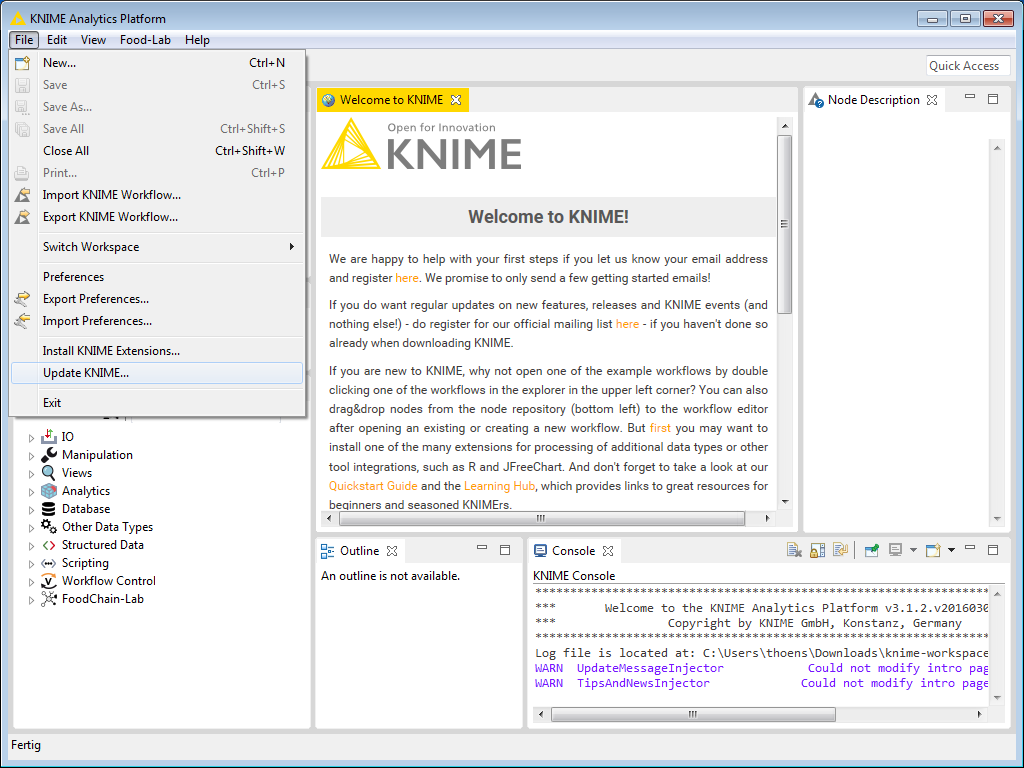
\includegraphics[height=0.6\textheight]{1.png}
	\end{center}
	\begin{itemize}
		\item Select \textbf{File $>$ Update KNIME...} in the menu bar.
	\end{itemize}
\end{frame}

\section{2}
\begin{frame}
	\begin{center}
  		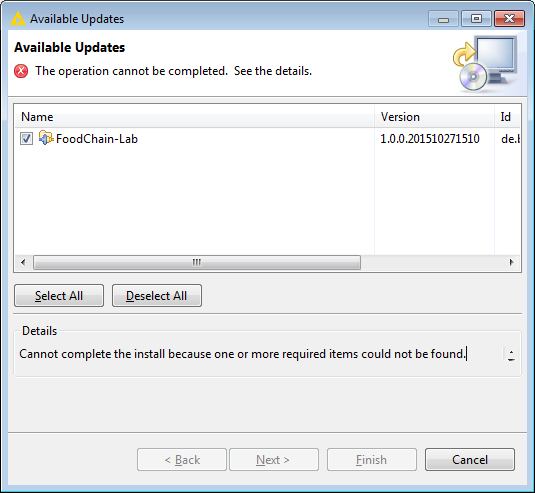
\includegraphics[height=0.6\textheight]{2.png}
	\end{center}
	\begin{itemize}
		\item If there is an update for only one KNIME extension, you will see this dialog.
		\item Press \textbf{Finish} and continue with step 6.
		\item Otherwise (if multiple updates are available) continue with step 3.
	\end{itemize}
\end{frame}

\section{3}
\begin{frame}
	\begin{center}
  		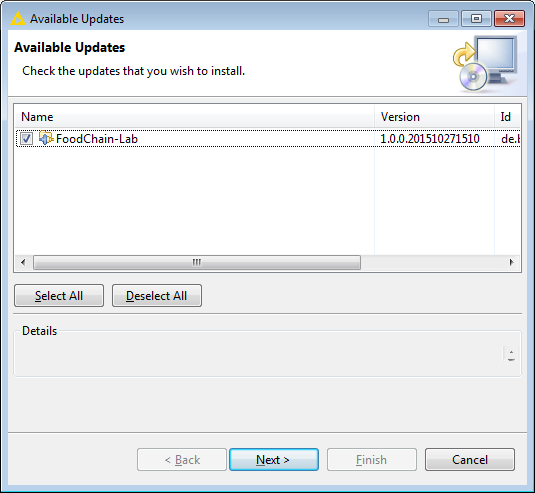
\includegraphics[height=0.6\textheight]{3.png}
	\end{center}
	\begin{itemize}
		\item This dialog lists all KNIME extensions, for which an update is available.
		\item Make sure that all items are checked and press \textbf{Next}.
	\end{itemize}
\end{frame}

\section{4}
\begin{frame}
	\begin{center}
  		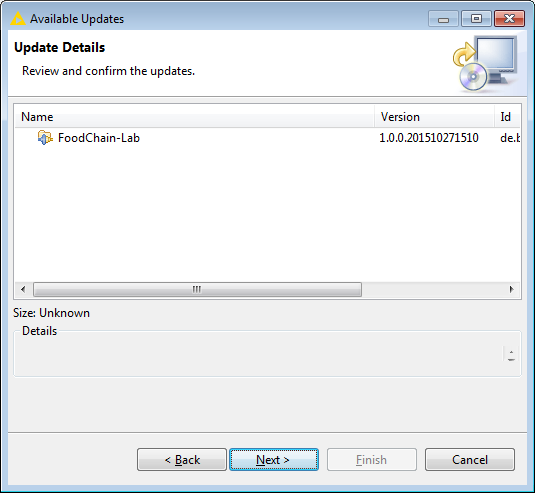
\includegraphics[height=0.6\textheight]{4.png}
	\end{center}
	\begin{itemize}
		\item In the next window, you’ll see a list of the tools to be downloaded. Click \textbf{Next}.
	\end{itemize}
\end{frame}

\section{5}
\begin{frame}
	\begin{center}
  		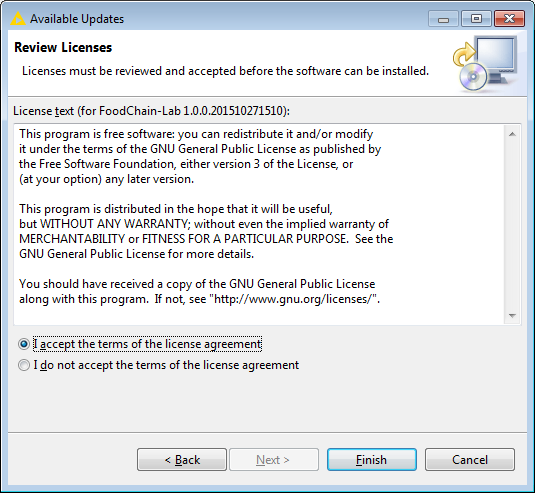
\includegraphics[height=0.6\textheight]{5.png}
	\end{center}
	\begin{itemize}
		\item Read and accept the license agreements, then click \textbf{Finish}.
	\end{itemize}
\end{frame}

\section{6}
\begin{frame}
	\begin{center}
  		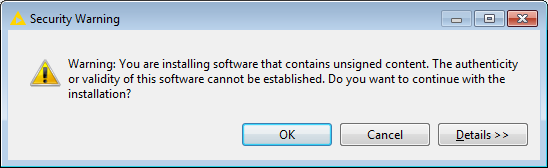
\includegraphics[width=0.7\textwidth]{6.png}
	\end{center}
	\begin{itemize}
		\item If you get a security warning saying that the authenticity or validity of the software can’t be established, click \textbf{OK}.
	\end{itemize}
\end{frame}

\section{7}
\begin{frame}
	\begin{center}
  		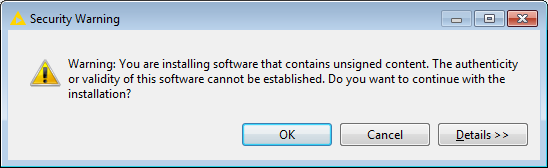
\includegraphics[width=0.7\textwidth]{7.png}
	\end{center}
	\begin{itemize}
		\item When the installation completes, restart KNIME.
	\end{itemize}
\end{frame}

\end{document}